%
\begin{isabellebody}%
\def\isabellecontext{Presentation}%
%
\isadelimtheory
%
\endisadelimtheory
%
\isatagtheory
\isacommand{theory}\isamarkupfalse%
\ Presentation\isanewline
\isakeyword{imports}\ Base\isanewline
\isakeyword{begin}%
\endisatagtheory
{\isafoldtheory}%
%
\isadelimtheory
%
\endisadelimtheory
%
\isamarkupchapter{Presenting theories \label{ch:present}%
}
\isamarkuptrue%
%
\begin{isamarkuptext}%
Isabelle provides several ways to present the outcome of formal
  developments, including WWW-based browsable libraries or actual
  printable documents.  Presentation is centered around the concept of
  \emph{logic sessions}.  The global session structure is that of a
  tree, with Isabelle Pure at its root, further object-logics derived
  (e.g.\ HOLCF from HOL, and HOL from Pure), and application sessions
  in leaf positions (usually without a separate image).

  The tools \indexref{}{tool}{mkdir}\hyperlink{tool.mkdir}{\mbox{\isa{\isatool{mkdir}}}} and \indexref{}{tool}{make}\hyperlink{tool.make}{\mbox{\isa{\isatool{make}}}} provide the primary
  means for managing Isabelle sessions, including proper setup for
  presentation.  Here \indexref{}{tool}{usedir}\hyperlink{tool.usedir}{\mbox{\isa{\isatool{usedir}}}} takes care to let
  \indexref{}{executable}{isabelle-process}\hyperlink{executable.isabelle-process}{\mbox{\isa{\isatt{isabelle{\isaliteral{2D}{\isacharminus}}process}}}} process run any additional
  stages required for document preparation, notably the tools
  \indexref{}{tool}{document}\hyperlink{tool.document}{\mbox{\isa{\isatool{document}}}} and \indexref{}{tool}{latex}\hyperlink{tool.latex}{\mbox{\isa{\isatool{latex}}}}.  The complete tool chain
  for managing batch-mode Isabelle sessions is illustrated in
  \figref{fig:session-tools}.

  \begin{figure}[htbp]
  \begin{center}
  \begin{tabular}{lp{0.6\textwidth}}

      \indexref{}{tool}{mkdir}\hyperlink{tool.mkdir}{\mbox{\isa{\isatool{mkdir}}}} & invoked once by the user to create the
      initial source setup (common \verb|IsaMakefile| plus a
      single session directory); \\

      \hyperlink{tool.make}{\mbox{\isa{\isatool{make}}}} & invoked repeatedly by the user to keep session
      output up-to-date (HTML, documents etc.); \\

      \hyperlink{tool.usedir}{\mbox{\isa{\isatool{usedir}}}} & part of the standard \verb|IsaMakefile|
      entry of a session; \\

      \hyperlink{executable.isabelle-process}{\mbox{\isa{\isatt{isabelle{\isaliteral{2D}{\isacharminus}}process}}}} & run through \indexref{}{tool}{usedir}\hyperlink{tool.usedir}{\mbox{\isa{\isatool{usedir}}}}; \\

      \indexref{}{tool}{document}\hyperlink{tool.document}{\mbox{\isa{\isatool{document}}}} & run by the Isabelle process if document
      preparation is enabled; \\

      \indexref{}{tool}{latex}\hyperlink{tool.latex}{\mbox{\isa{\isatool{latex}}}} & universal {\LaTeX} tool wrapper invoked
      multiple times by \indexref{}{tool}{document}\hyperlink{tool.document}{\mbox{\isa{\isatool{document}}}}; also useful for manual
      experiments; \\

  \end{tabular}
  \caption{The tool chain of Isabelle session presentation} \label{fig:session-tools}
  \end{center}
  \end{figure}%
\end{isamarkuptext}%
\isamarkuptrue%
%
\isamarkupsection{Generating theory browser information \label{sec:info}%
}
\isamarkuptrue%
%
\begin{isamarkuptext}%
\index{theory browsing information|bold}

  As a side-effect of running a logic sessions, Isabelle is able to
  generate theory browsing information, including HTML documents that
  show a theory's definition, the theorems proved in its ML file and
  the relationship with its ancestors and descendants.  Besides the
  HTML file that is generated for every theory, Isabelle stores links
  to all theories in an index file. These indexes are linked with
  other indexes to represent the overall tree structure of logic
  sessions.

  Isabelle also generates graph files that represent the theory
  hierarchy of a logic.  There is a graph browser Java applet embedded
  in the generated HTML pages, and also a stand-alone application that
  allows browsing theory graphs without having to start a WWW client
  first.  The latter version also includes features such as generating
  Postscript files, which are not available in the applet version.
  See \secref{sec:browse} for further information.

  \medskip

  The easiest way to let Isabelle generate theory browsing information
  for existing sessions is to append ``\verb|-i true|'' to the
  \indexref{}{setting}{ISABELLE\_USEDIR\_OPTIONS}\hyperlink{setting.ISABELLE-USEDIR-OPTIONS}{\mbox{\isa{\isatt{ISABELLE{\isaliteral{5F}{\isacharunderscore}}USEDIR{\isaliteral{5F}{\isacharunderscore}}OPTIONS}}}} before invoking \hyperlink{tool.make}{\mbox{\isa{\isatool{make}}}}.
  For example, add something like this to your Isabelle settings file

\begin{ttbox}
ISABELLE_USEDIR_OPTIONS="-i true"
\end{ttbox}

  and then change into the \verb|~~/src/FOL| directory and run
  \hyperlink{tool.make}{\mbox{\isa{\isatool{make}}}}, or even \hyperlink{tool.make}{\mbox{\isa{\isatool{make}}}}~\verb|all|.  The
  presentation output will appear in \verb|ISABELLE_BROWSER_INFO/FOL|, which usually refers to something like
  \verb|~/.isabelle/IsabelleXXXX/browser_info/FOL|.  Note that
  option \verb|-v true| will make the internal runs of \hyperlink{tool.usedir}{\mbox{\isa{\isatool{usedir}}}} more explicit about such details.

  Many standard Isabelle sessions (such as \verb|~~/src/HOL/ex|)
  also provide actual printable documents.  These are prepared
  automatically as well if enabled like this, using the \verb|-d| option
\begin{ttbox}
ISABELLE_USEDIR_OPTIONS="-i true -d dvi"
\end{ttbox}
  Enabling options \verb|-i| and \verb|-d|
  simultaneously as shown above causes an appropriate ``document''
  link to be included in the HTML index.  Documents (or raw document
  sources) may be generated independently of browser information as
  well, see \secref{sec:tool-document} for further details.

  \bigskip The theory browsing information is stored in a
  sub-directory directory determined by the \indexref{}{setting}{ISABELLE\_BROWSER\_INFO}\hyperlink{setting.ISABELLE-BROWSER-INFO}{\mbox{\isa{\isatt{ISABELLE{\isaliteral{5F}{\isacharunderscore}}BROWSER{\isaliteral{5F}{\isacharunderscore}}INFO}}}} setting plus a prefix corresponding to the
  session identifier (according to the tree structure of sub-sessions
  by default).  A complete WWW view of all standard object-logics and
  examples of the Isabelle distribution is available at the usual
  Isabelle sites:
  \begin{center}\small
  \begin{tabular}{l}
    \url{http://isabelle.in.tum.de/dist/library/} \\
    \url{http://www.cl.cam.ac.uk/research/hvg/Isabelle/dist/library/} \\
    \url{http://mirror.cse.unsw.edu.au/pub/isabelle/dist/library/} \\
  \end{tabular}
  \end{center}
  
  \medskip In order to present your own theories on the web, simply
  copy the corresponding subdirectory from \hyperlink{setting.ISABELLE-BROWSER-INFO}{\mbox{\isa{\isatt{ISABELLE{\isaliteral{5F}{\isacharunderscore}}BROWSER{\isaliteral{5F}{\isacharunderscore}}INFO}}}} to your WWW server, having generated browser
  info like this:
\begin{ttbox}
isabelle usedir -i true HOL Foo
\end{ttbox}

  This assumes that directory \verb|Foo| contains some \verb|ROOT.ML| file to load all your theories, and HOL is your parent
  logic image (\indexref{}{tool}{mkdir}\hyperlink{tool.mkdir}{\mbox{\isa{\isatool{mkdir}}}} assists in setting up Isabelle
  session directories.  Theory browser information for HOL should have
  been generated already beforehand.  Alternatively, one may specify
  an external link to an existing body of HTML data by giving \hyperlink{tool.usedir}{\mbox{\isa{\isatool{usedir}}}} a \verb|-P| option like this:
\begin{ttbox}
isabelle usedir -i true -P http://isabelle.in.tum.de/library/ HOL Foo
\end{ttbox}

  \medskip For production use, \hyperlink{tool.usedir}{\mbox{\isa{\isatool{usedir}}}} is usually invoked in an
  appropriate \verb|IsaMakefile|, via \hyperlink{tool.make}{\mbox{\isa{\isatool{make}}}}.  There is a
  separate \hyperlink{tool.mkdir}{\mbox{\isa{\isatool{mkdir}}}} tool to provide easy setup of all this, with
  only minimal manual editing required.
\begin{ttbox}
isabelle mkdir HOL Foo && isabelle make
\end{ttbox}
  See \secref{sec:tool-mkdir} for more information on preparing
  Isabelle session directories, including the setup for documents.%
\end{isamarkuptext}%
\isamarkuptrue%
%
\isamarkupsection{Creating Isabelle session directories
  \label{sec:tool-mkdir}%
}
\isamarkuptrue%
%
\begin{isamarkuptext}%
The \indexdef{}{tool}{mkdir}\hypertarget{tool.mkdir}{\hyperlink{tool.mkdir}{\mbox{\isa{\isatool{mkdir}}}}} tool prepares Isabelle session source
  directories, including a sensible default setup of \verb|IsaMakefile|, \verb|ROOT.ML|, and a \verb|document|
  directory with a minimal \verb|root.tex| that is sufficient to
  print all theories of the session (in the order of appearance); see
  \secref{sec:tool-document} for further information on Isabelle
  document preparation.  The usage of \hyperlink{tool.mkdir}{\mbox{\isa{\isatool{mkdir}}}} is:

\begin{ttbox}
Usage: isabelle mkdir [OPTIONS] [LOGIC] NAME

  Options are:
    -I FILE      alternative IsaMakefile output
    -P           include parent logic target
    -b           setup build mode (session outputs heap image)
    -q           quiet mode

  Prepare session directory, including IsaMakefile and document source,
  with parent LOGIC (default ISABELLE_LOGIC=\$ISABELLE_LOGIC)
\end{ttbox}

  The \hyperlink{tool.mkdir}{\mbox{\isa{\isatool{mkdir}}}} tool is conservative in the sense that any
  existing \verb|IsaMakefile| etc.\ is left unchanged.  Thus it
  is safe to invoke it multiple times, although later runs may not
  have the desired effect.

  Note that \hyperlink{tool.mkdir}{\mbox{\isa{\isatool{mkdir}}}} is unable to change \verb|IsaMakefile|
  incrementally --- manual changes are required for multiple
  sub-sessions.  On order to get an initial working session, the only
  editing needed is to add appropriate \verb|use_thy| calls to the
  generated \verb|ROOT.ML| file.%
\end{isamarkuptext}%
\isamarkuptrue%
%
\isamarkupsubsubsection{Options%
}
\isamarkuptrue%
%
\begin{isamarkuptext}%
The \verb|-I| option specifies an alternative to \verb|IsaMakefile| for dependencies.  Note that ``\verb|-|'' refers
  to \emph{stdout}, i.e.\ ``\verb|-I-|'' provides an easy way
  to peek at \hyperlink{tool.mkdir}{\mbox{\isa{\isatool{mkdir}}}}'s idea of \hyperlink{tool.make}{\mbox{\isa{\isatool{make}}}} setup required for
  some particular of Isabelle session.

  \medskip The \verb|-P| option includes a target for the
  parent \verb|LOGIC| session in the generated \verb|IsaMakefile|.  The corresponding sources are assumed to be located
  within the Isabelle distribution.

  \medskip The \verb|-b| option sets up the current directory
  as the base for a new session that provides an actual logic image,
  as opposed to one that only runs several theories based on an
  existing image.  Note that in the latter case, everything except
  \verb|IsaMakefile| would be placed into a separate directory
  \verb|NAME|, rather than the current one.  See
  \secref{sec:tool-usedir} for further information on \emph{build
  mode} vs.\ \emph{example mode} of \hyperlink{tool.usedir}{\mbox{\isa{\isatool{usedir}}}}.

  \medskip The \verb|-q| option enables quiet mode, suppressing
  further notes on how to proceed.%
\end{isamarkuptext}%
\isamarkuptrue%
%
\isamarkupsubsubsection{Examples%
}
\isamarkuptrue%
%
\begin{isamarkuptext}%
The standard setup of a single ``example session'' based on the
  default logic, with proper document generation is generated like
  this:
\begin{ttbox}
isabelle mkdir Foo && isabelle make
\end{ttbox}

  \noindent The theory sources should be put into the \verb|Foo|
  directory, and its \verb|ROOT.ML| should be edited to load all
  required theories.  Invoking \hyperlink{tool.make}{\mbox{\isa{\isatool{make}}}} again would run the whole
  session, generating browser information and the document
  automatically.  The \verb|IsaMakefile| is typically tuned
  manually later, e.g.\ adding source dependencies, or changing the
  options passed to \hyperlink{tool.usedir}{\mbox{\isa{\isatool{usedir}}}}.

  \medskip Large projects may demand further sessions, potentially
  with separate logic images being created.  This usually requires
  manual editing of the generated \verb|IsaMakefile|, which is
  meant to cover all of the sub-session directories at the same time
  (this is the deeper reasong why \verb|IsaMakefile| is not made
  part of the initial session directory created by \hyperlink{tool.mkdir}{\mbox{\isa{\isatool{mkdir}}}}).
  See \verb|~~/src/HOL/IsaMakefile| for a full-blown example.%
\end{isamarkuptext}%
\isamarkuptrue%
%
\isamarkupsection{Running Isabelle sessions \label{sec:tool-usedir}%
}
\isamarkuptrue%
%
\begin{isamarkuptext}%
The \indexdef{}{tool}{usedir}\hypertarget{tool.usedir}{\hyperlink{tool.usedir}{\mbox{\isa{\isatool{usedir}}}}} tool builds object-logic images, or
  runs example sessions based on existing logics. Its usage is:
\begin{ttbox}
Usage: isabelle usedir [OPTIONS] LOGIC NAME

  Options are:
    -C BOOL      copy existing document directory to -D PATH (default true)
    -D PATH      dump generated document sources into PATH
    -M MAX       multithreading: maximum number of worker threads (default 1)
    -P PATH      set path for remote theory browsing information
    -Q INT       set threshold for sub-proof parallelization (default 50)
    -T LEVEL     multithreading: trace level (default 0)
    -V VARIANT   declare alternative document VARIANT
    -b           build mode (output heap image, using current dir)
    -d FORMAT    build document as FORMAT (default false)
    -f NAME      use ML file NAME (default ROOT.ML)
    -g BOOL      generate session graph image for document (default false)
    -i BOOL      generate theory browser information (default false)
    -m MODE      add print mode for output
    -p LEVEL     set level of detail for proof objects (default 0)
    -q LEVEL     set level of parallel proof checking (default 1)
    -r           reset session path
    -s NAME      override session NAME
    -t BOOL      internal session timing (default false)
    -v BOOL      be verbose (default false)

  Build object-logic or run examples. Also creates browsing
  information (HTML etc.) according to settings.

  ISABELLE_USEDIR_OPTIONS=...

  ML_PLATFORM=...
  ML_HOME=...
  ML_SYSTEM=...
  ML_OPTIONS=...
\end{ttbox}

  Note that the value of the \indexref{}{setting}{ISABELLE\_USEDIR\_OPTIONS}\hyperlink{setting.ISABELLE-USEDIR-OPTIONS}{\mbox{\isa{\isatt{ISABELLE{\isaliteral{5F}{\isacharunderscore}}USEDIR{\isaliteral{5F}{\isacharunderscore}}OPTIONS}}}}
  setting is implicitly prefixed to \emph{any} \hyperlink{tool.usedir}{\mbox{\isa{\isatool{usedir}}}}
  call. Since the \verb|IsaMakefile|s of all object-logics
  distributed with Isabelle just invoke \hyperlink{tool.usedir}{\mbox{\isa{\isatool{usedir}}}} for the real
  work, one may control compilation options globally via above
  variable. In particular, generation of \rmindex{HTML} browsing
  information and document preparation is controlled here.%
\end{isamarkuptext}%
\isamarkuptrue%
%
\isamarkupsubsubsection{Options%
}
\isamarkuptrue%
%
\begin{isamarkuptext}%
Basically, there are two different modes of operation: \emph{build
  mode} (enabled through the \verb|-b| option) and
  \emph{example mode} (default).

  Calling \hyperlink{tool.usedir}{\mbox{\isa{\isatool{usedir}}}} with \verb|-b| runs \hyperlink{executable.isabelle-process}{\mbox{\isa{\isatt{isabelle{\isaliteral{2D}{\isacharminus}}process}}}} with input image \verb|LOGIC| and output to
  \verb|NAME|, as provided on the command line. This will be a
  batch session, running \verb|ROOT.ML| from the current
  directory and then quitting.  It is assumed that \verb|ROOT.ML|
  contains all ML commands required to build the logic.

  In example mode, \hyperlink{tool.usedir}{\mbox{\isa{\isatool{usedir}}}} runs a read-only session of
  \verb|LOGIC| and automatically runs \verb|ROOT.ML| from
  within directory \verb|NAME|.  It assumes that this file
  contains appropriate ML commands to run the desired examples.

  \medskip The \verb|-i| option controls theory browser data
  generation. It may be explicitly turned on or off --- as usual, the
  last occurrence of \verb|-i| on the command line wins.

  The \verb|-P| option specifies a path (or actual URL) to be
  prefixed to any \emph{non-local} reference of existing theories.
  Thus user sessions may easily link to existing Isabelle libraries
  already present on the WWW.

  The \verb|-m| options specifies additional print modes to be
  activated temporarily while the session is processed.

  \medskip The \verb|-d| option controls document preparation.
  Valid arguments are \verb|false| (do not prepare any document;
  this is default), or any of \verb|dvi|, \verb|dvi.gz|,
  \verb|ps|, \verb|ps.gz|, \verb|pdf|.  The logic
  session has to provide a properly setup \verb|document|
  directory.  See \secref{sec:tool-document} and
  \secref{sec:tool-latex} for more details.

  \medskip The \verb|-V| option declares alternative document
  variants, consisting of name/tags pairs (cf.\ options \verb|-n| and \verb|-t| of \indexref{}{tool}{document}\hyperlink{tool.document}{\mbox{\isa{\isatool{document}}}}).  The standard
  document is equivalent to ``\verb|document=theory,proof,ML|'', which means that all theory begin/end
  commands, proof body texts, and ML code will be presented
  faithfully.

  An alternative variant ``\verb|outline=/proof/ML|'' would
  fold proof and ML parts, replacing the original text by a short
  place-holder.  The form ``\isa{name}\verb|=-|,'' means to
  remove document \isa{name} from the list of variants to be
  processed.  Any number of \verb|-V| options may be given;
  later declarations have precedence over earlier ones.

  Some document variant \isa{name} may use an alternative {\LaTeX}
  entry point called \verb|document/root_|\isa{{\isaliteral{22}{\isachardoublequote}}name{\isaliteral{22}{\isachardoublequote}}}\verb|.tex| if that file exists; otherwise the common
  \verb|document/root.tex| is used.

  \medskip The \verb|-g| option produces images of the theory
  dependency graph (cf.\ \secref{sec:browse}) for inclusion in the
  generated document, both as \verb|session_graph.eps| and
  \verb|session_graph.pdf| at the same time.  To include this in
  the final {\LaTeX} document one could say \verb|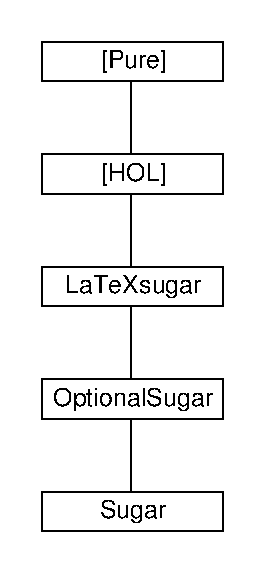
\includegraphics{session_graph}| in \verb|document/root.tex| (omitting the file-name extension enables
  {\LaTeX} to select to correct version, either for the DVI or PDF
  output path).

  \medskip The \verb|-D| option causes the generated document
  sources to be dumped at location \verb|PATH|; this path is
  relative to the session's main directory.  If the \verb|-C|
  option is true, this will include a copy of an existing \verb|document| directory as provided by the user.  For example, \hyperlink{tool.usedir}{\mbox{\isa{\isatool{usedir}}}}~\verb|-D generated HOL Foo| produces a complete set
  of document sources at \verb|Foo/generated|.  Subsequent
  invocation of \hyperlink{tool.document}{\mbox{\isa{\isatool{document}}}}~\verb|Foo/generated| (see also
  \secref{sec:tool-document}) will process the final result
  independently of an Isabelle job.  This decoupled mode of operation
  facilitates debugging of serious {\LaTeX} errors, for example.

  \medskip The \verb|-p| option determines the level of detail
  for internal proof objects, see also the \emph{Isabelle Reference
  Manual}~\cite{isabelle-ref}.

  \medskip The \verb|-q| option specifies the level of parallel
  proof checking: \verb|0| no proofs, \verb|1| toplevel
  proofs (default), \verb|2| toplevel and nested Isar proofs.
  The option \verb|-Q| specifies a threshold for \verb|-q2|: nested proofs are only parallelized when the current number
  of forked proofs falls below the given value (default 50),
  multiplied by the number of worker threads (see option \verb|-M|).

  \medskip The \verb|-t| option produces a more detailed
  internal timing report of the session.

  \medskip The \verb|-v| option causes additional information
  to be printed while running the session, notably the location of
  prepared documents.

  \medskip The \verb|-M| option specifies the maximum number of
  parallel worker threads used for processing independent tasks when
  checking theory sources (multithreading only works on suitable ML
  platforms).  The special value of \verb|0| or \verb|max|
  refers to the number of actual CPU cores of the underlying machine,
  which is a good starting point for optimal performance tuning.  The
  \verb|-T| option determines the level of detail in tracing
  output concerning the internal locking and scheduling in
  multithreaded operation.  This may be helpful in isolating
  performance bottle-necks, e.g.\ due to excessive wait states when
  locking critical code sections.

  \medskip Any \hyperlink{tool.usedir}{\mbox{\isa{\isatool{usedir}}}} session is named by some \emph{session
  identifier}. These accumulate, documenting the way sessions depend
  on others. For example, consider \verb|Pure/FOL/ex|, which
  refers to the examples of FOL, which in turn is built upon Pure.

  The current session's identifier is by default just the base name of
  the \verb|LOGIC| argument (in build mode), or of the \verb|NAME| argument (in example mode). This may be overridden explicitly
  via the \verb|-s| option.%
\end{isamarkuptext}%
\isamarkuptrue%
%
\isamarkupsubsubsection{Examples%
}
\isamarkuptrue%
%
\begin{isamarkuptext}%
Refer to the \verb|IsaMakefile|s of the Isabelle
  distribution's object-logics as a model for your own developments.
  For example, see \verb|~~/src/FOL/IsaMakefile|.  The \indexref{}{tool}{mkdir}\hyperlink{tool.mkdir}{\mbox{\isa{\isatool{mkdir}}}} tool creates \verb|IsaMakefile|s with proper invocation
  of \hyperlink{tool.usedir}{\mbox{\isa{\isatool{usedir}}}} as well.%
\end{isamarkuptext}%
\isamarkuptrue%
%
\isamarkupsection{Preparing Isabelle session documents
  \label{sec:tool-document}%
}
\isamarkuptrue%
%
\begin{isamarkuptext}%
The \indexdef{}{tool}{document}\hypertarget{tool.document}{\hyperlink{tool.document}{\mbox{\isa{\isatool{document}}}}} tool prepares logic session
  documents, processing the sources both as provided by the user and
  generated by Isabelle.  Its usage is:
\begin{ttbox}
Usage: isabelle document [OPTIONS] [DIR]

  Options are:
    -c           cleanup -- be aggressive in removing old stuff
    -n NAME      specify document name (default 'document')
    -o FORMAT    specify output format: dvi (default), dvi.gz, ps,
                 ps.gz, pdf
    -t TAGS      specify tagged region markup

  Prepare the theory session document in DIR (default 'document')
  producing the specified output format.
\end{ttbox}
  This tool is usually run automatically as part of the corresponding
  Isabelle batch process, provided document preparation has been
  enabled (cf.\ the \verb|-d| option of \indexref{}{tool}{usedir}\hyperlink{tool.usedir}{\mbox{\isa{\isatool{usedir}}}}).
  It may be manually invoked on the generated browser information
  document output as well, e.g.\ in case of errors encountered in the
  batch run.

  \medskip The \verb|-c| option tells \hyperlink{tool.document}{\mbox{\isa{\isatool{document}}}} to
  dispose the document sources after successful operation.  This is
  the right thing to do for sources generated by an Isabelle process,
  but take care of your files in manual document preparation!

  \medskip The \verb|-n| and \verb|-o| option specify
  the final output file name and format, the default is ``\verb|document.dvi|''.  Note that the result will appear in the parent of
  the target \verb|DIR|.

  \medskip The \verb|-t| option tells {\LaTeX} how to interpret
  tagged Isabelle command regions.  Tags are specified as a comma
  separated list of modifier/name pairs: ``\verb|+|\isa{foo}'' (or just ``\isa{foo}'') means to keep, ``\verb|-|\isa{foo}'' to drop, and ``\verb|/|\isa{foo}'' to
  fold text tagged as \isa{foo}.  The builtin default is equivalent
  to the tag specification ``\verb|+theory,+proof,+ML,+visible,-invisible|''; see also the {\LaTeX}
  macros \verb|\isakeeptag|, \verb|\isadroptag|, and
  \verb|\isafoldtag|, in \verb|~~/lib/texinputs/isabelle.sty|.

  \medskip Document preparation requires a properly setup ``\verb|document|'' directory within the logic session sources.  This
  directory is supposed to contain all the files needed to produce the
  final document --- apart from the actual theories which are
  generated by Isabelle.

  \medskip For most practical purposes, \hyperlink{tool.document}{\mbox{\isa{\isatool{document}}}} is smart
  enough to create any of the specified output formats, taking
  \verb|root.tex| supplied by the user as a starting point.  This
  even includes multiple runs of {\LaTeX} to accommodate references
  and bibliographies (the latter assumes \verb|root.bib| within
  the same directory).

  In more complex situations, a separate \verb|IsaMakefile| for
  the document sources may be given instead.  This should provide
  targets for any admissible document format; these have to produce
  corresponding output files named after \verb|root| as well,
  e.g.\ \verb|root.dvi| for target format \verb|dvi|.

  \medskip When running the session, Isabelle copies the content of
  the original \verb|document| directory into its proper place
  within \hyperlink{setting.ISABELLE-BROWSER-INFO}{\mbox{\isa{\isatt{ISABELLE{\isaliteral{5F}{\isacharunderscore}}BROWSER{\isaliteral{5F}{\isacharunderscore}}INFO}}}}, according to the session
  path and document variant.  Then, for any processed theory \isa{A}
  some {\LaTeX} source is generated and put there as \isa{A}\verb|.tex|.  Furthermore, a list of all generated theory
  files is put into \verb|session.tex|.  Typically, the root
  {\LaTeX} file provided by the user would include \verb|session.tex| to get a document containing all the theories.

  The {\LaTeX} versions of the theories require some macros defined in
  \verb|~~/lib/texinputs/isabelle.sty|.  Doing \verb|\usepackage{isabelle}| in \verb|root.tex| should be fine;
  the underlying \hyperlink{tool.latex}{\mbox{\isa{\isatool{latex}}}} already includes an appropriate path
  specification for {\TeX} inputs.

  If the text contains any references to Isabelle symbols (such as
  \verb|\|\verb|<forall>|) then \verb|isabellesym.sty| should be included as well.  This package
  contains a standard set of {\LaTeX} macro definitions \verb|\isasym|\isa{foo} corresponding to \verb|\|\verb|<|\isa{foo}\verb|>|, see \cite{isabelle-implementation} for a
  complete list of predefined Isabelle symbols.  Users may invent
  further symbols as well, just by providing {\LaTeX} macros in a
  similar fashion as in \verb|~~/lib/texinputs/isabellesym.sty| of
  the distribution.

  For proper setup of DVI and PDF documents (with hyperlinks and
  bookmarks), we recommend to include \verb|~~/lib/texinputs/pdfsetup.sty| as well.

  \medskip As a final step of document preparation within Isabelle,
  \hyperlink{tool.document}{\mbox{\isa{\isatool{document}}}}~\verb|-c| is run on the resulting \verb|document| directory.  Thus the actual output document is built and
  installed in its proper place (as linked by the session's \verb|index.html| if option \verb|-i| of \indexref{}{tool}{usedir}\hyperlink{tool.usedir}{\mbox{\isa{\isatool{usedir}}}} has
  been enabled, cf.\ \secref{sec:info}).  The generated sources are
  deleted after successful run of {\LaTeX} and friends.  Note that a
  separate copy of the sources may be retained by passing an option
  \verb|-D| to \hyperlink{tool.usedir}{\mbox{\isa{\isatool{usedir}}}} when running the session.%
\end{isamarkuptext}%
\isamarkuptrue%
%
\isamarkupsection{Running {\LaTeX} within the Isabelle environment
  \label{sec:tool-latex}%
}
\isamarkuptrue%
%
\begin{isamarkuptext}%
The \indexdef{}{tool}{latex}\hypertarget{tool.latex}{\hyperlink{tool.latex}{\mbox{\isa{\isatool{latex}}}}} tool provides the basic interface for
  Isabelle document preparation.  Its usage is:
\begin{ttbox}
Usage: isabelle latex [OPTIONS] [FILE]

  Options are:
    -o FORMAT    specify output format: dvi (default), dvi.gz, ps,
                 ps.gz, pdf, bbl, idx, sty, syms

  Run LaTeX (and related tools) on FILE (default root.tex),
  producing the specified output format.
\end{ttbox}

  Appropriate {\LaTeX}-related programs are run on the input file,
  according to the given output format: \hyperlink{executable.latex}{\mbox{\isa{\isatt{latex}}}},
  \hyperlink{executable.pdflatex}{\mbox{\isa{\isatt{pdflatex}}}}, \hyperlink{executable.dvips}{\mbox{\isa{\isatt{dvips}}}}, \hyperlink{executable.bibtex}{\mbox{\isa{\isatt{bibtex}}}}
  (for \verb|bbl|), and \hyperlink{executable.makeindex}{\mbox{\isa{\isatt{makeindex}}}} (for \verb|idx|).  The actual commands are determined from the settings
  environment (\hyperlink{setting.ISABELLE-LATEX}{\mbox{\isa{\isatt{ISABELLE{\isaliteral{5F}{\isacharunderscore}}LATEX}}}} etc.).

  The \verb|sty| output format causes the Isabelle style files to
  be updated from the distribution.  This is useful in special
  situations where the document sources are to be processed another
  time by separate tools (cf.\ option \verb|-D| of \hyperlink{tool.usedir}{\mbox{\isa{\isatool{usedir}}}}).

  The \verb|syms| output is for internal use; it generates lists
  of symbols that are available without loading additional {\LaTeX}
  packages.%
\end{isamarkuptext}%
\isamarkuptrue%
%
\isamarkupsubsubsection{Examples%
}
\isamarkuptrue%
%
\begin{isamarkuptext}%
Invoking \hyperlink{tool.latex}{\mbox{\isa{\isatool{latex}}}} by hand may be occasionally useful when
  debugging failed attempts of the automatic document preparation
  stage of batch-mode Isabelle.  The abortive process leaves the
  sources at a certain place within \hyperlink{setting.ISABELLE-BROWSER-INFO}{\mbox{\isa{\isatt{ISABELLE{\isaliteral{5F}{\isacharunderscore}}BROWSER{\isaliteral{5F}{\isacharunderscore}}INFO}}}},
  see the runtime error message for details.  This enables users to
  inspect {\LaTeX} runs in further detail, e.g.\ like this:

\begin{ttbox}
  cd ~/.isabelle/IsabelleXXXX/browser_info/HOL/Test/document
  isabelle latex -o pdf
\end{ttbox}%
\end{isamarkuptext}%
\isamarkuptrue%
%
\isadelimtheory
%
\endisadelimtheory
%
\isatagtheory
\isacommand{end}\isamarkupfalse%
%
\endisatagtheory
{\isafoldtheory}%
%
\isadelimtheory
%
\endisadelimtheory
\end{isabellebody}%
%%% Local Variables:
%%% mode: latex
%%% TeX-master: "root"
%%% End:
